% !TeX program = lualatex
% !TeX spellcheck = uk_UA

\documentclass[14pt, a4paper]{extarticle}

% -- Мови та шрифти (згідно з ДСТУ) --
\usepackage{fontspec}
\usepackage[english, ukrainian]{babel}
\usepackage{csquotes}

\setmainfont{Times New Roman}
\setsansfont{Arial}
\setmonofont{Courier New}[Scale=0.85]

% -- Математичні пакети --
\usepackage{amsmath, amssymb, mathtools}

% -- Оптимізація тексту для LuaLaTeX --
\usepackage[protrusion=true, expansion=true]{microtype}
\emergencystretch=3.5em
\hbadness=10000

% -- Параметри сторінки згідно з ДСТУ 3008:2015 --
\usepackage[
    left=30mm,
    right=15mm,
    top=20mm,
    bottom=20mm,
    footskip=10mm,
    headheight=17pt
]{geometry}

% -- Міжрядковий інтервал (еквівалент 1.5 Word) та абзацний відступ --
\linespread{1.3}
\usepackage{indentfirst}
\setlength{\parindent}{1.25cm}
\setlength{\parskip}{0pt}

% -- Колонтитули та нумерація сторінок (вгорі праворуч, без лінійок) --
\usepackage{fancyhdr}
\fancypagestyle{plain}{
    \fancyhf{}
    \rhead{\thepage}
    \renewcommand{\headrulewidth}{0pt}
}
\pagestyle{plain}

% -- Форматування заголовків згідно з ДСТУ 3008:2015 --
\usepackage[explicit]{titlesec}

% Формат розділів (14pt, напівжирний, абзацний відступ 1.25cm)
\titleformat{\section}[block]
{\normalsize\bfseries\raggedright}
{\thesection\ }
{0pt}
{#1}
\titlespacing*{\section}{\parindent}{14pt}{7pt}

% Формат підрозділів
\titleformat{\subsection}[block]
{\normalsize\bfseries\raggedright}
{\thesubsection\ }
{0pt}
{#1}
\titlespacing*{\subsection}{\parindent}{14pt}{7pt}

% -- Списки (компактні, вирівняні за абзацним відступом) --
\usepackage{enumitem}
\setlist{
    nosep,
    leftmargin=*,
    labelindent=\parindent
}
\setlist[itemize]{label=--}

% -- Підписи до рисунків та таблиць згідно з ДСТУ 3008:2015 --
\usepackage{caption}
\DeclareCaptionLabelSeparator{emdash}{ -- }

\captionsetup[figure]{
    labelsep=emdash,
    name={Рисунок},
    justification=centering,
    position=bottom,
    font=normalsize
}

\captionsetup[table]{
    labelsep=emdash,
    name={Таблиця},
    justification=raggedright,
    singlelinecheck=false,
    position=top,
    font=normalsize
}

% -- Таблиці (книжковий стиль, нормальний інтервал) --
\usepackage{booktabs}
\usepackage{tabularx}
\usepackage{multirow}
\newcolumntype{Y}{>{\raggedright\arraybackslash}X}
\renewcommand{\arraystretch}{1.0}

% -- Графіка та гіперпосилання --
\usepackage{graphicx}
\usepackage[hidelinks]{hyperref}

% -- Завантаження модуля обробки таблиць Lua --
\directlua{dofile("tables.lua")}

\begin{document}

% -- Титульна сторінка --
\begin{titlepage}
    \thispagestyle{empty}
    \setlength{\parindent}{0pt}
    
    % -- ШАПКА ДОКУМЕНТА (12pt, напівжирний) --
    \begin{center}
        {\fontsize{12pt}{16pt}\selectfont\bfseries
        МІНІСТЕРСТВО ОСВІТИ І НАУКИ УКРАЇНИ\\[3pt]
        ОДЕСЬКИЙ НАЦІОНАЛЬНИЙ УНІВЕРСИТЕТ ІМЕНІ І.І. МЕЧНИКОВА\\[3pt]
        ФАКУЛЬТЕТ МАТЕМАТИКИ, ФІЗИКИ ТА ІНФОРМАЦІЙНИХ ТЕХНОЛОГІЙ\\[3pt]
        КАФЕДРА ОПТИМАЛЬНОГО КЕРУВАННЯ ТА ЕКОНОМІЧНОЇ КІБЕРНЕТИКИ\par}
    \end{center}

    \vspace{1.5cm}

    % -- НАЗВА РОБОТИ ТА ТЕМА --
    \begin{center}
        {\fontsize{18pt}{22pt}\selectfont\bfseries ЗВІТ\\
        до лабораторної роботи № 7\par}
        \vspace{0.4cm}
        {\fontsize{14pt}{18pt}\selectfont
        з дисципліни «Системи комп’ютерного зору»\par}
        \vspace{0.4cm}
        {\fontsize{16pt}{20pt}\selectfont\bfseries
        на тему:\\[6pt]
        «Сегментація, класичний детектор, оцінювання якості»\par}
    \end{center}

    \vspace{1.5cm}

    % -- ПРАВИЙ БЛОК (Виконавець) --
    \hfill
    \begin{minipage}{0.60\textwidth}
        \raggedright
        {\fontsize{14pt}{19pt}\selectfont
        Виконав:\\[2pt]
        студент 3 курсу групи 1\\[2pt]
        спеціальності F1 «Прикладна математика»\\[2pt]
        Касьянов Ярослав Володимирович
        }
    \end{minipage}

    \vfill

    % -- МІСТО ТА РІК --
    \begin{center}
        {\fontsize{12pt}{14pt}\selectfont\bfseries Одеса -- 2026\par}
    \end{center}
\end{titlepage}

% За ДСТУ титульна сторінка входить у загальну нумерацію як 1-ша,
% тому наступна сторінка отримує номер 2:
\setcounter{page}{2}


\section{Мета роботи}
Порівняти класичні методи бінарної сегментації зображень (порогування Оцу, маркерний вододіл, суперпікселі \texttt{SLIC} із колірною кластеризацією та \texttt{GrabCut}) на власному розміченому наборі з 10 зображень за метриками $\text{IoU}$ і Дайса з аналізом розкиду, продемонструвати оманливість піксельної точності за дисбалансу класів, а також реалізувати повний конвеєр оцінювання класичного детектора пішоходів \texttt{HOG+SVM} із власним немаксимальним придушенням (\texttt{NMS}), кривою \emph{precision--recall} та обчисленням середньої точності ($\text{AP}$).

\section{Вихідні дані}
\begin{itemize}
    \item \textbf{Власний набір сегментації (\texttt{lab07/data/part\_a})}: 10 фотографій з одним помітним об'єктом на кожній ($4032 \times 2268$ або $2268 \times 4032$~пк, робочий масштаб обробки $0.25\times$: $1008 \times 567$ / $567 \times 1008$~пк) та 10 відповідних ручних масок у форматі PNG (\texttt{1.png}--\texttt{10.png}, \texttt{1\_mask.png}--\texttt{10\_mask.png}). Набір збалансовано включає 5 складних сцен із неоднорідним фоном, відблисками або малим об'єктом (№~1--5) та 5 сцен із контрастним однотонним фоном (№~6--10); на трьох кадрах (№~3, 9, 10) об'єкт займає менше $10\%$ площі.
    \item \textbf{Набір для детекції пішоходів (\texttt{lab07/data/part\_e/Test})}: перші 30 анотованих зображень тестової вибірки відкритого набору \emph{INRIA Person} у форматі Pascal VOC XML, що містять сумарно $86$ еталонних рамок класу \texttt{person}.
    \item \textbf{Програмне забезпечення}: Python~3.13, OpenCV~5.0 (\texttt{cv2}), scikit-image~0.26 (\texttt{skimage.segmentation.slic}), NumPy, Matplotlib; стан генератора випадкових чисел зафіксовано (\texttt{np.random.seed(42)}).
\end{itemize}

\section{Теоретичні відомості}
\begin{enumerate}
    \item \textbf{Порогування Оцу, вододіл, \texttt{SLIC} і \texttt{GrabCut}}: метод Оцу обирає глобальний поріг $t^*$, що максимізує міжкласову дисперсію яскравостей фону ($0$) і переднього плану ($1$):
    \begin{equation}\label{eq:otsu}
        t^* = \arg\max_{t} \, \sigma_B^2(t) = \arg\max_{t} \, \omega_0(t)\,\omega_1(t)\bigl(\mu_0(t) - \mu_1(t)\bigr)^2.
    \end{equation}
    Маркерний вододіл інтерпретує градієнт зображення як рельєф і затоплює басейни від достовірних маркерів, отриманих через перетворення відстані; \texttt{SLIC} групує пікселі у компактні суперпікселі у $5$-вимірному просторі $(L, a, b, x, y)$; \texttt{GrabCut} ітеративно оптимізує енергію Гіббса $E(\boldsymbol{\alpha}) = U(\boldsymbol{\alpha}, \boldsymbol{\theta}) + V(\boldsymbol{\alpha})$ розрізом графа (\emph{min-cut}) з гауссівськими сумішами кольорів (GMM) переднього плану та фону.

    \item \textbf{Метрики якості сегментації ($\text{IoU}$, Дайс, піксельна точність)}: для прогнозованої маски $P$ та еталонної маски $G$ через кількість пікселів $\text{TP}, \text{FP}, \text{FN}, \text{TN}$ обчислюються:
    \begin{equation}\label{eq:seg_metrics}
        \text{IoU} = \frac{|P \cap G|}{|P \cup G|} = \frac{\text{TP}}{\text{TP} + \text{FP} + \text{FN}}, \quad
        \text{Dice} = \frac{2|P \cap G|}{|P| + |G|} = \frac{2\,\text{IoU}}{1 + \text{IoU}},
    \end{equation}
    \begin{equation}\label{eq:acc}
        \text{Accuracy} = \frac{\text{TP} + \text{TN}}{\text{TP} + \text{TN} + \text{FP} + \text{FN}}.
    \end{equation}
    За малого об'єкта ($|G| \ll |I|$) домінування $\text{TN}$ робить $\text{Accuracy} \approx 1 - |G|/|I| > 90\%$ навіть для тривіальної порожньої маски ($P = \varnothing$), тоді як $\text{IoU} = 0$.

    \item \textbf{Оцінювання детектора (\texttt{NMS}, \emph{precision--recall} та $\text{AP}$)}: для впорядкованих за спаданням впевненості виявлень після немаксимального придушення ($\text{IoU} > 0.5$) та зіставлення з еталоном ($\text{IoU} \ge 0.5$, один еталон -- одне співставлення) будуються кумулятивні точність $P(k) = \frac{\text{TP}_k}{\text{TP}_k + \text{FP}_k}$, повнота $R(k) = \frac{\text{TP}_k}{N_{\text{GT}}}$, монотонна огинаюча $P_{\text{env}}(r)$ та середня точність $\text{AP}$:
    \begin{equation}\label{eq:ap}
        P_{\text{env}}(r) = \max_{\tilde{r} \ge r} P(\tilde{r}), \qquad
        \text{AP} = \sum_{n} \bigl(R_n - R_{n-1}\bigr)\,P_{\text{env}}(R_n).
    \end{equation}
\end{enumerate}

\section{Хід роботи}

\subsection{Частина A. Розмітка та перевірка масок (Кроки 1--2)}
\begin{itemize}
    \item \textbf{Кроки 1--2}: Завантажено 10 власних зображень та їхні ручні маски. Програмна перевірка підтвердила точний збіг розмірів кожної пари зображення--маска ($4032 \times 2268$ або $2268 \times 4032$~пк). Оскільки вихідні маски з графічного редактора містили згладжування контуру ($163$--$256$ проміжних рівнів сірого у форматі RGBA), їх приведено порогом $> 127$ до строго бінарного одноканального подання з рівно двома рівнями $\{0, 255\}$ і збережено у \texttt{results/masks\_binary/} (Таблиця~\ref{tab:dataset_masks}, Рис.~\ref{fig:dataset_overview}).
\end{itemize}

\subsection{Частина B. Порівняння чотирьох методів сегментації (Кроки 3--7)}
\begin{itemize}
    \item \textbf{Крок 3 (Оцу)}: На масштабі $0.25\times$ виконано згладжування $5 \times 5$ та глобальну бінаризацію \texttt{cv2.threshold(..., THRESH\_OTSU)} з автоматичним визначенням полярності за межею кадру (периметр $5\%$ вважається фоном).
    \item \textbf{Крок 4 (Вододіл із маркерами)}: Послідовно виконано 7 етапів практикуму: Оцу $\to$ морфологічне відкриття еліпсом $3 \times 3$ (2 ітерації) $\to$ \texttt{cv2.distanceTransform} ($L_2$) $\to$ поріг $0.5 \cdot d_{\max}$ для певного переднього плану $\to$ дилатація (3 ітерації) для зони фону $\to$ \texttt{cv2.connectedComponents} $\to$ \texttt{cv2.watershed}.
    \item \textbf{Крок 5 (\texttt{SLIC})}: Застосовано \texttt{skimage.segmentation.slic} (\texttt{n\_segments=400}, \texttt{compactness=10}), обчислено середні кольори суперпікселів у просторі CIE~Lab та об'єднано їх у два класи методом \texttt{cv2.kmeans} ($k = 2$) з тією ж орієнтацією полярності за периметром.
    \item \textbf{Кроки 6--7 (\texttt{GrabCut} і метрики)}: Виконано \texttt{cv2.grabCut} ($5$ ітерацій, прямокутник із відступом $12$~пк навколо об'єкта). Власними функціями обчислено $\text{IoU}$ та коефіцієнт Дайса для всіх $10 \times 4$ експериментів і зведено середнє, стандартне відхилення, мінімум і максимум (Таблиці~\ref{tab:methods_summary}--\ref{tab:per_image_iou}, Рис.~\ref{fig:seg_comparison}--\ref{fig:metrics_boxplot}).
\end{itemize}

\subsection{Частина C. Демонстрація оманливості точності (Крок 8)}
\begin{itemize}
    \item \textbf{Крок 8}: Відібрано всі три зображення набору з площею об'єкта менше $10\%$: №~3 (карта microSD, $0.75\%$), №~10 (біла картка, $6.25\%$) і №~9 (подвійна розетка, $7.33\%$). Для порожньої маски ($P = \varnothing$) обчислено піксельну точність і $\text{IoU}$ та зіставлено з результатами Оцу й \texttt{GrabCut} (Таблиця~\ref{tab:accuracy_paradox}, Рис.~\ref{fig:accuracy_paradox}).
\end{itemize}

\subsection{Частина D. Узгодженість між розмітниками (Кроки 9--10)}
\begin{itemize}
    \item \textbf{Кроки 9--10 (статус виконання)}: У скрипті \texttt{src/part\_a\_b\_c\_d.py} реалізовано автоматичне обчислення міжрозмітникових метрик $\text{IoU}$ та Дайса при появі незалежної розмітки колеги у каталозі \texttt{lab07/data/part\_d/}. На поточний момент друга (незалежна) маска ще не передана, тому числовий результат Частини~D має статус очікування (після додавання файлу колеги таблиця та оцінка верхньої межі якості перераховуються автоматично).
\end{itemize}

\subsection{Частина E. Детектор пішоходів \texttt{HOG+SVM} і крива \emph{precision--recall} (Кроки 11--16)}
\begin{itemize}
    \item \textbf{Кроки 11--13}: Ініціалізовано \texttt{cv2.HOGDescriptor()} зі стандартним детектором пішоходів \texttt{getDefaultPeopleDetector()} та запущено \texttt{detectMultiScale} (\texttt{hitThreshold=-0.20}, \texttt{winStride=(4,4)}, \texttt{padding=(8,8)}, \texttt{scale=1.05}, \texttt{groupThreshold=0}) на 30 кадрах \emph{INRIA Person Test} ($86$ еталонів). Застосовано компенсацію вбудованих контекстних полів тренувального вікна Dalal--Triggs $64 \times 128$ ($16\%$ по ширині, $10\%$ по висоті) та власну реалізацію \texttt{NMS} ($\text{IoU} > 0.5$), що скоротила $8257$ сирих рамок до $579$ ($14.3\times$).
    \item \textbf{Кроки 14--16}: Реалізовано власне зіставлення з еталоном ($\text{IoU} \ge 0.5$, унікальне співставлення), побудову кривої \emph{precision--recall} та інтегрування $\text{AP}$ з монотонною огинаючою. Попередня перевірка функції $\text{AP}$ на тестовій послідовності лекції~8 ($N_{\text{GT}}=4$, $[\text{TP}, \text{TP}, \text{FP}, \text{FP}, \text{TP}]$) повернула точне значення $\mathbf{0.6500}$. Для кількісного аналізу порівняно 4 режими: основний конвеєр, без \texttt{NMS}, без сортування за впевненістю та без корекції контекстних полів (Таблиці~\ref{tab:hog_summary}--\ref{tab:pr_thresholds}, Рис.~\ref{fig:pr_curve}--\ref{fig:hog_detections}).
\end{itemize}

\newpage
\section{Результати}

\begin{table}[htbp]
\centering
\caption{Характеристики 10 власних зображень та перевірка бінарних масок (Частина A, Кроки 1--2)}
\label{tab:dataset_masks}
\scriptsize
\setlength{\tabcolsep}{3.5pt}
\begin{tabularx}{\textwidth}{c Y c c c c r}
\toprule
№ & Об'єкт та сцена & Тип фону & Розмір, пк & Збіг розміру & Рівні до $\to$ після & Площа об'єкта \\
\midrule
\directlua{tab_dataset_masks()}
\bottomrule
\end{tabularx}
\end{table}

\begin{figure}[htbp]
    \centering
    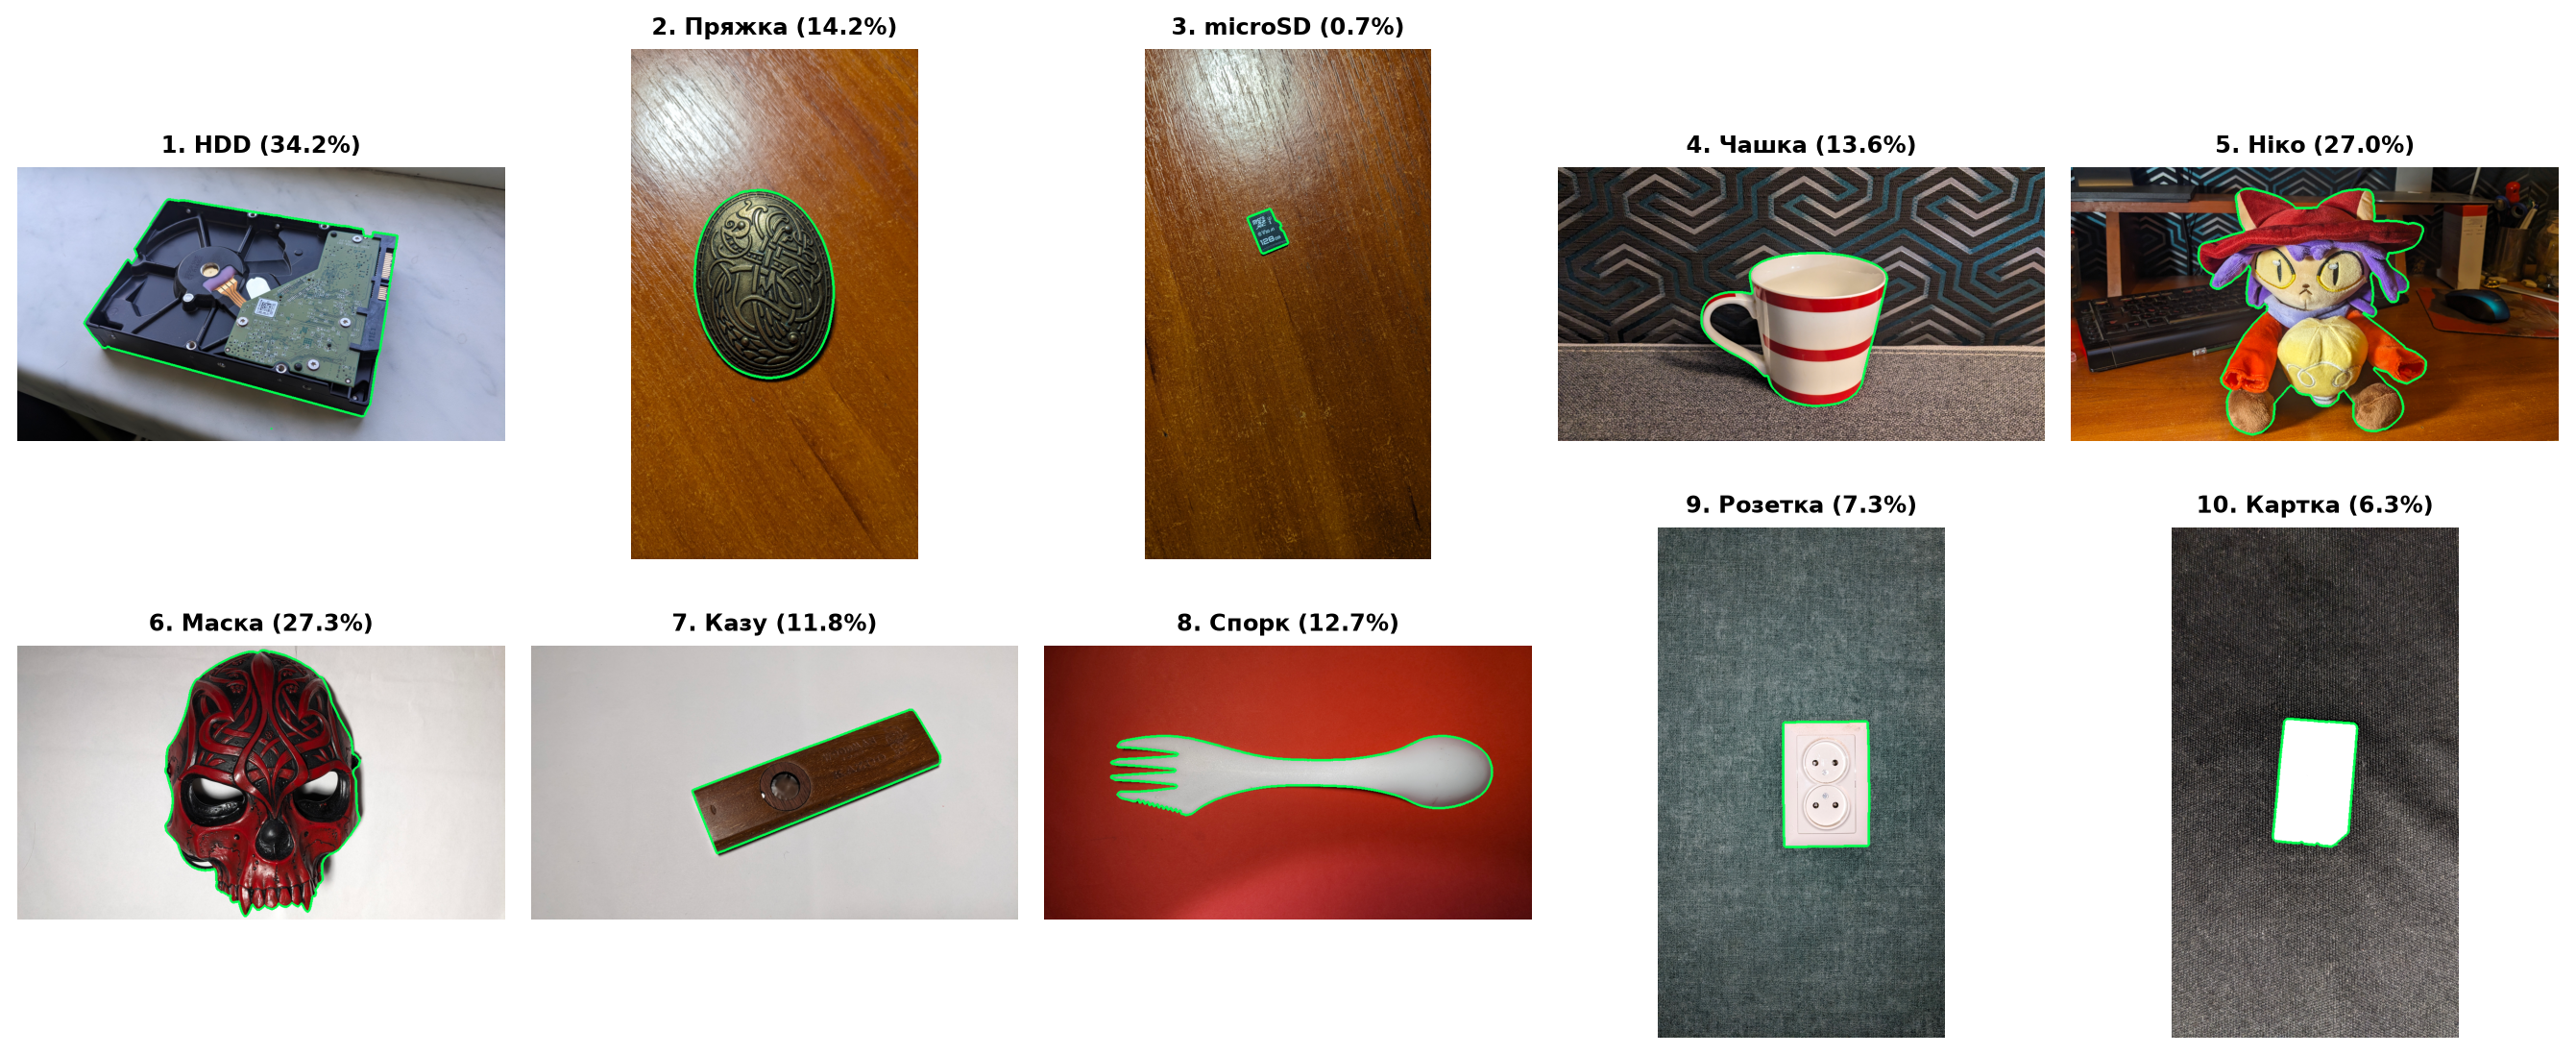
\includegraphics[width=0.98\textwidth]{../figures/a_dataset_overview.png}
    \caption{Власний набір із 10 зображень із накладеними контурами ручних еталонних масок (зелена лінія) та часткою площі об'єкта у кадрі (Кроки 1--2)}
    \label{fig:dataset_overview}
\end{figure}

\begin{table}[htbp]
\centering
\caption{Зведене порівняння чотирьох методів сегментації на 10 зображеннях (Частина B, Крок 7)}
\label{tab:methods_summary}
\scriptsize
\setlength{\tabcolsep}{3.8pt}
\begin{tabularx}{\textwidth}{Y r r r r r r}
\toprule
Метод сегментації & Середній $\text{IoU}$ & Стд. відх. $\sigma$ & Мін. $\text{IoU}$ & Макс. $\text{IoU}$ & Середній Dice & Сер. час/кадр \\
\midrule
\directlua{tab_methods_summary()}
\bottomrule
\end{tabularx}
\end{table}

\begin{table}[htbp]
\centering
\caption{Пооб'єктне порівняння метрики $\text{IoU}$ чотирьох методів сегментації (Частина B, Кроки 3--7)}
\label{tab:per_image_iou}
\scriptsize
\setlength{\tabcolsep}{3.8pt}
\begin{tabularx}{\textwidth}{c Y r r r r r}
\toprule
№ & Зображення (об'єкт і фон) & Площа & Оцу & Вододіл & \texttt{SLIC} & \texttt{GrabCut} \\
\midrule
\directlua{tab_per_image_iou()}
\bottomrule
\end{tabularx}
\end{table}

\begin{figure}[htbp]
    \centering
    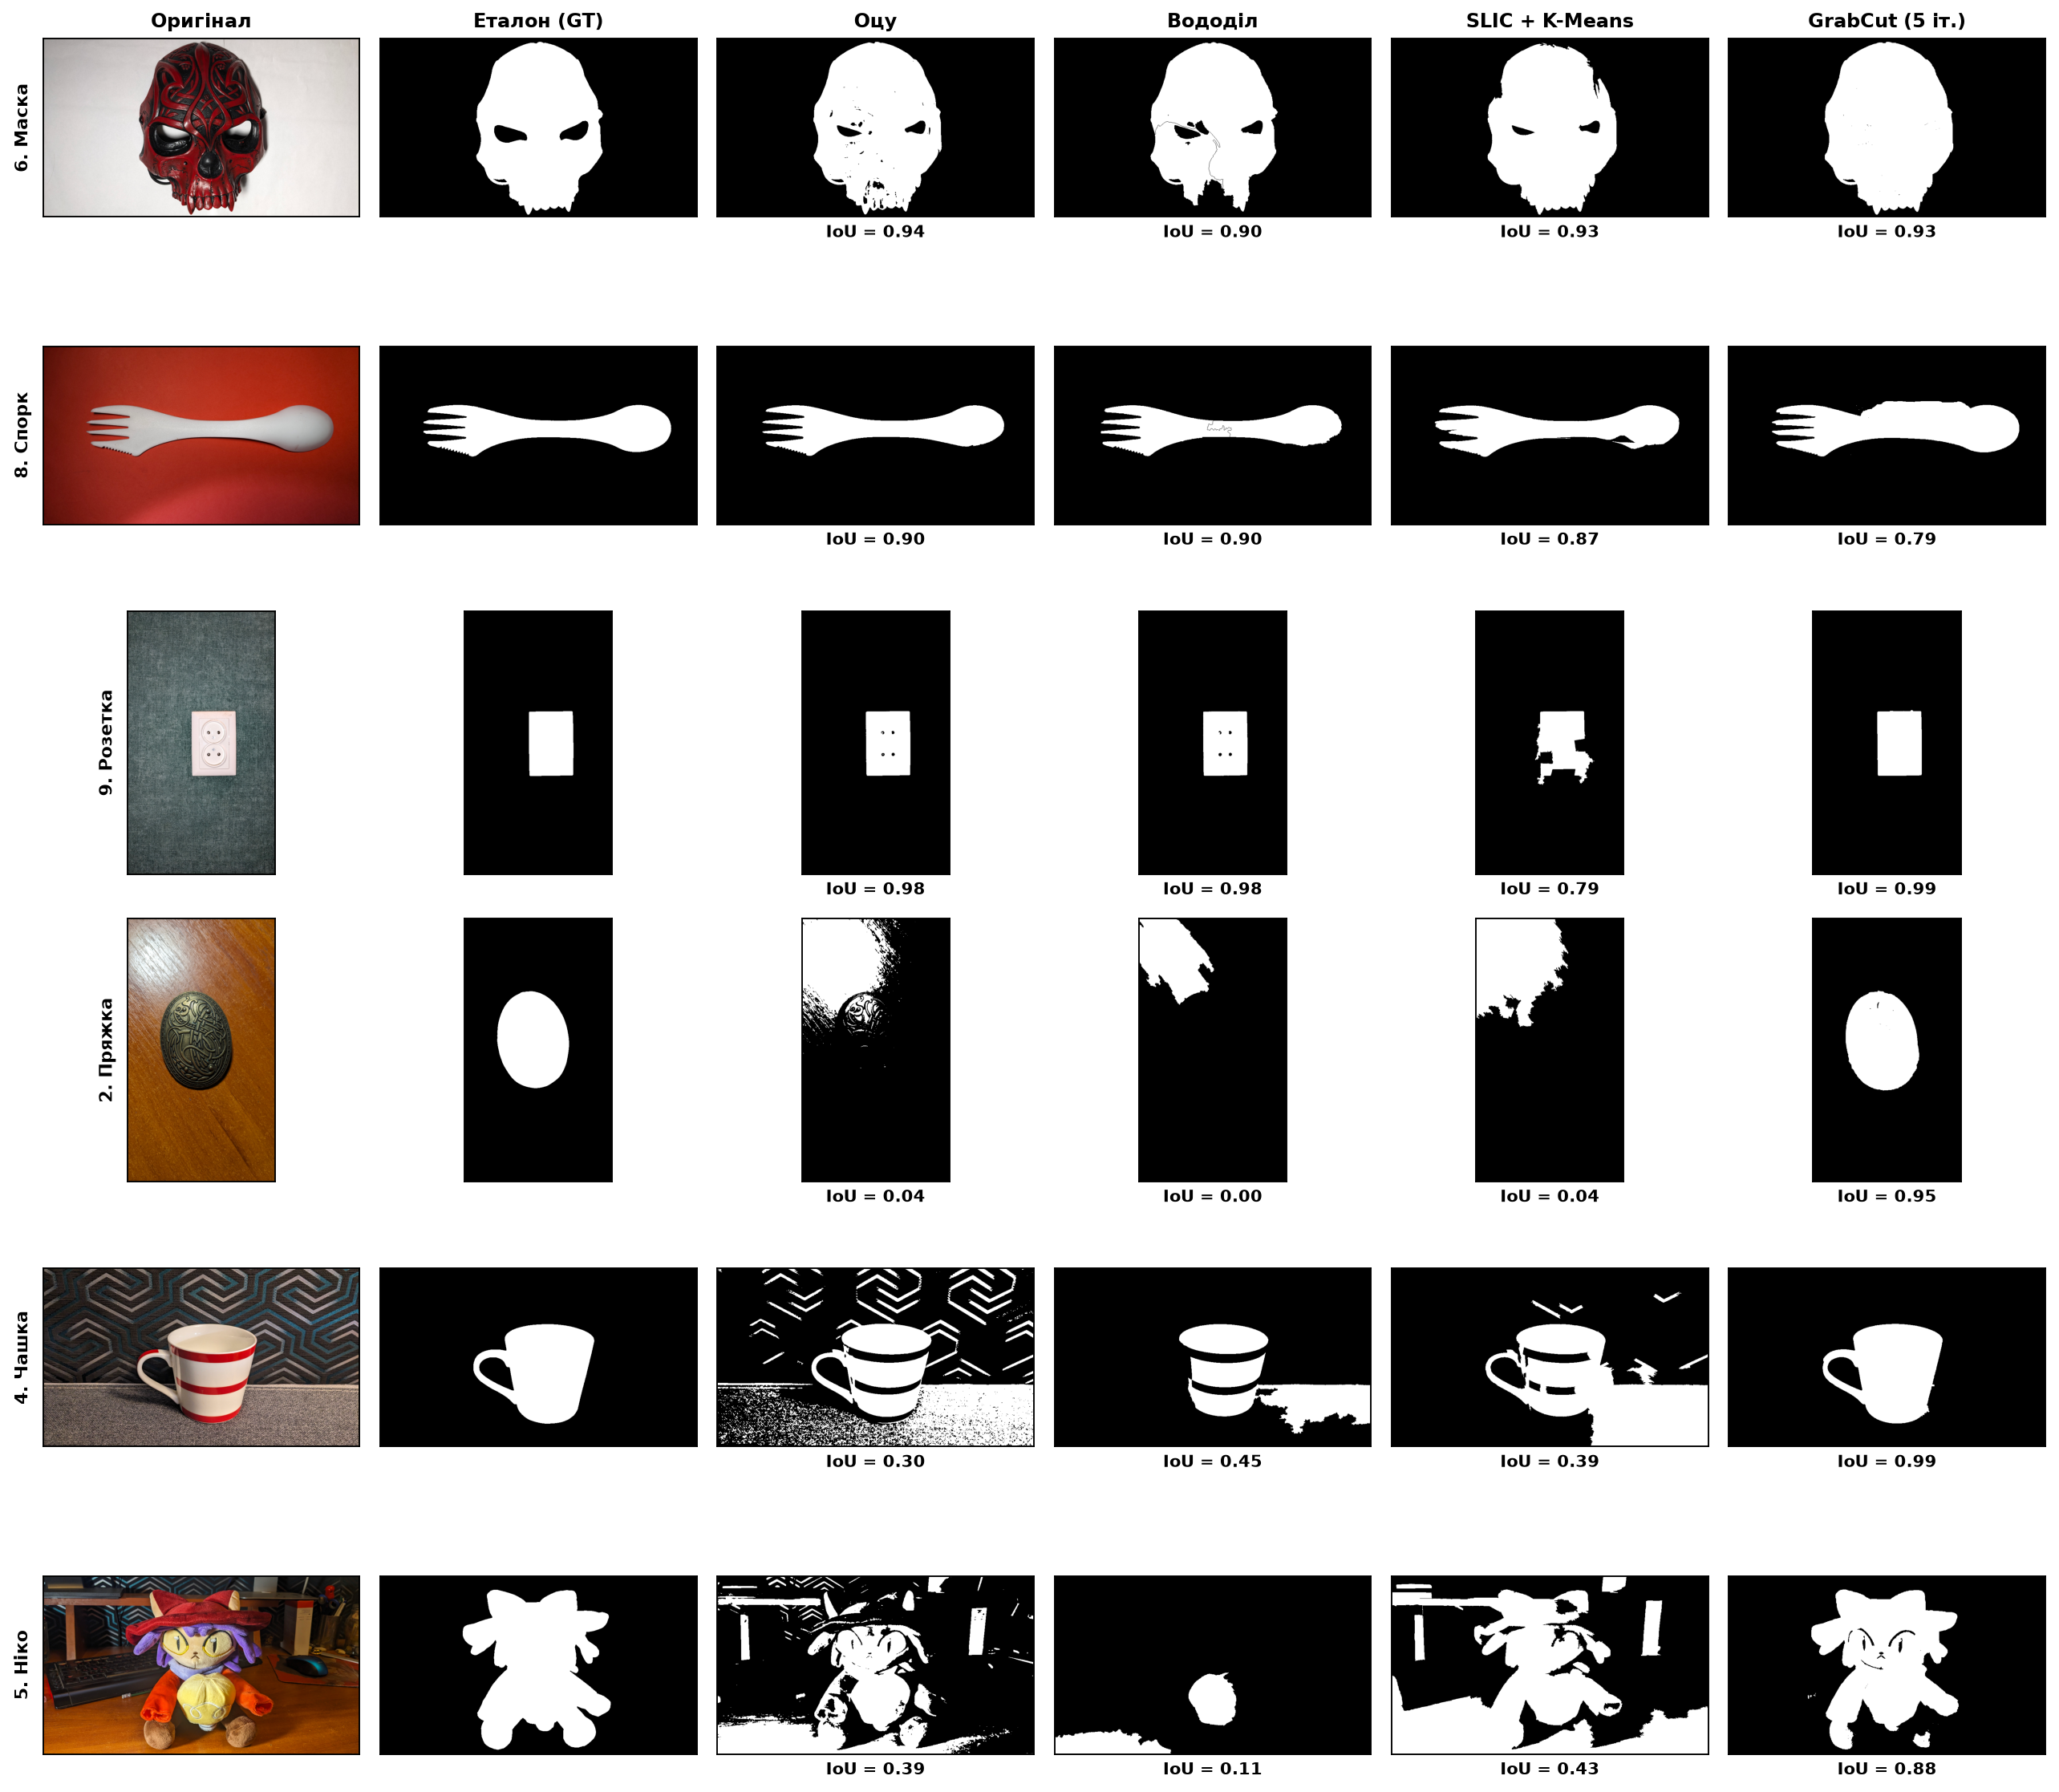
\includegraphics[width=0.97\textwidth]{../figures/b_segmentation_comparison.png}
    \caption{Візуальне порівняння масок чотирьох методів сегментації на контрастних (№~6, 8, 9) та складних (№~2, 4, 5) сценах із зазначенням $\text{IoU}$ (Кроки 3--7)}
    \label{fig:seg_comparison}
\end{figure}

\begin{figure}[htbp]
    \centering
    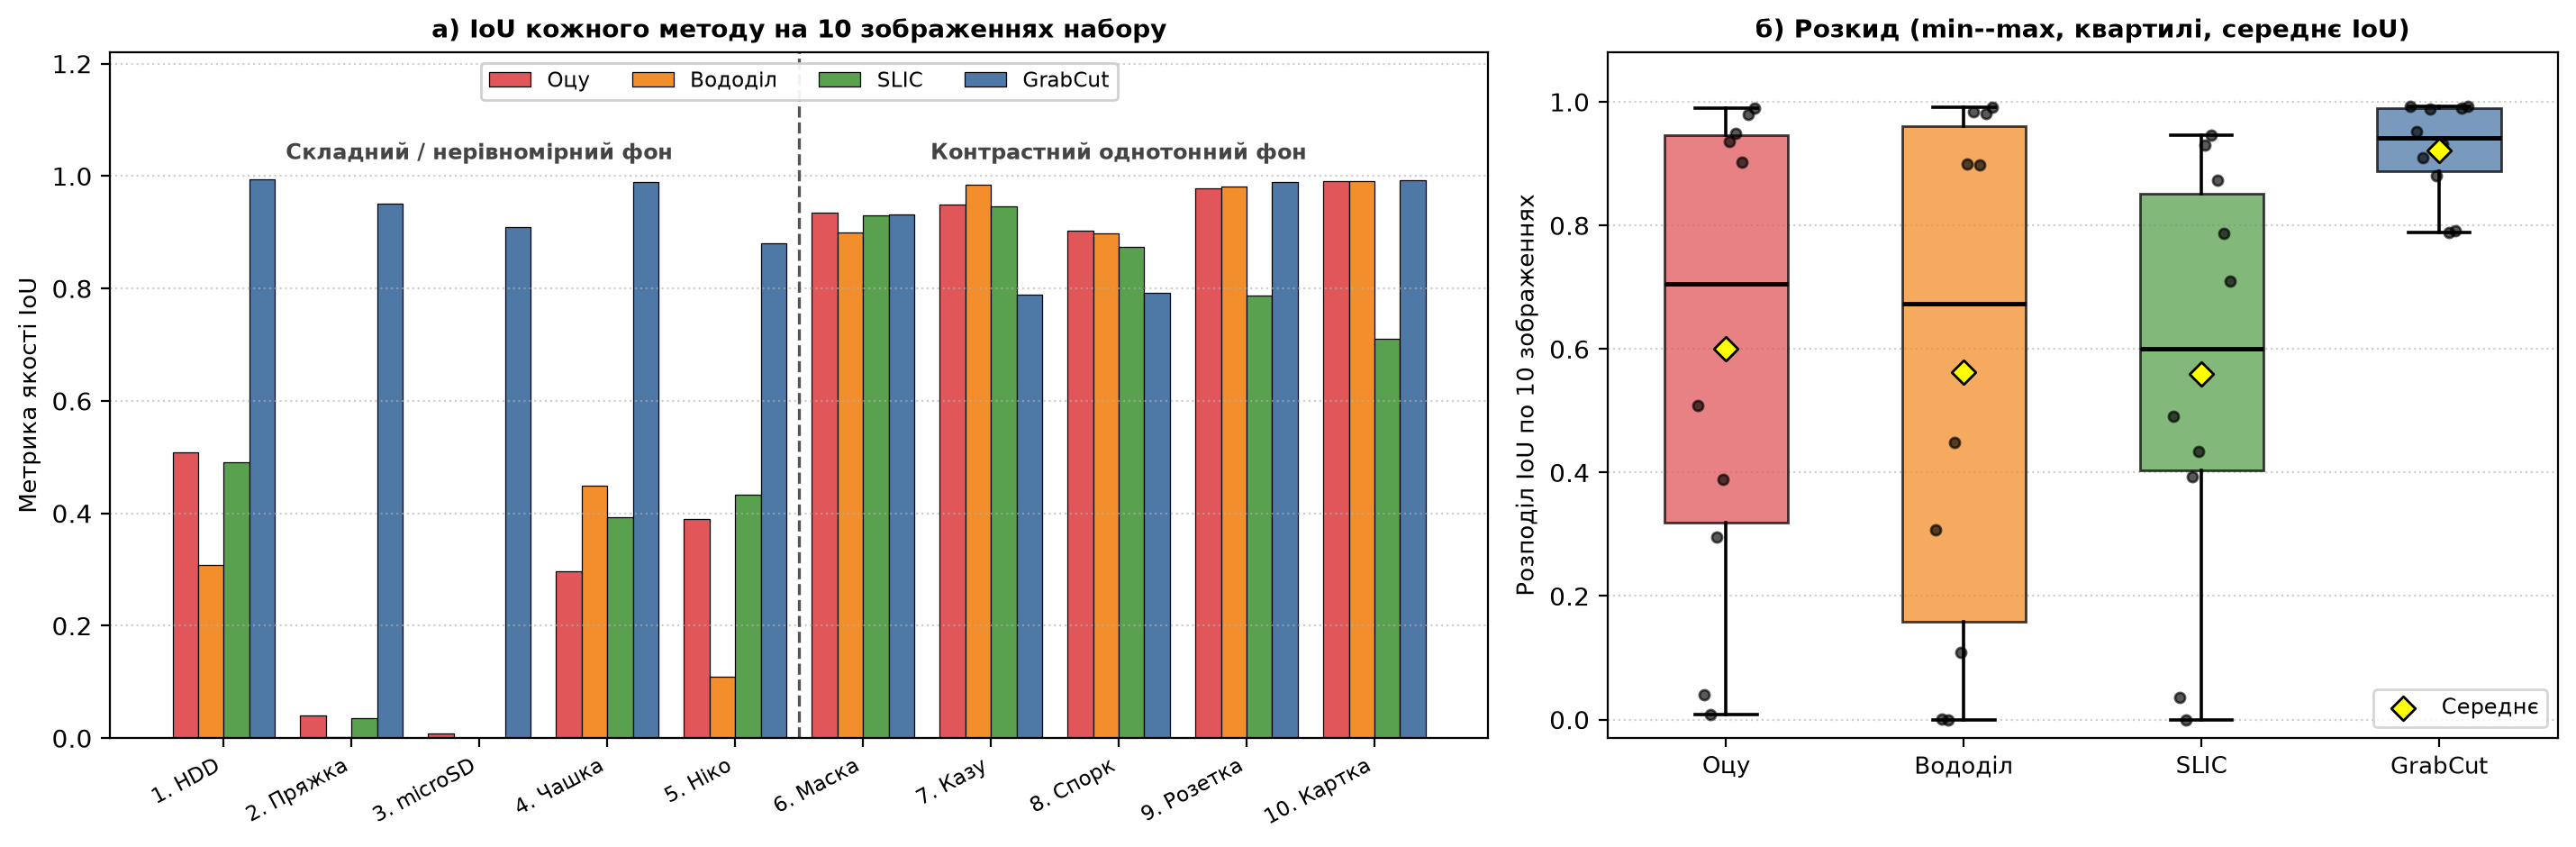
\includegraphics[width=0.98\textwidth]{../figures/b_metrics_boxplot.png}
    \caption{Кількісний розподіл якості сегментації (Крок 7): (а) $\text{IoU}$ кожного методу по всіх 10 кадрах із поділом за типом фону; (б) діаграма розкиду (мінімум, квартилі, медіана, середнє, максимум)}
    \label{fig:metrics_boxplot}
\end{figure}

\begin{table}[htbp]
\centering
\caption{Демонстрація оманливості піксельної точності на об'єктах площею $<10\%$ (Частина C, Крок 8)}
\label{tab:accuracy_paradox}
\scriptsize
\setlength{\tabcolsep}{3.2pt}
\begin{tabularx}{\textwidth}{c Y r r r c c}
\toprule
№ & Зображення (площа $<10\%$) & Площа & Порожня: Acc & Порожня: $\text{IoU}$ & Оцу: Acc / $\text{IoU}$ & \texttt{GrabCut}: Acc / $\text{IoU}$ \\
\midrule
\directlua{tab_accuracy_paradox()}
\bottomrule
\end{tabularx}
\end{table}

\begin{figure}[htbp]
    \centering
    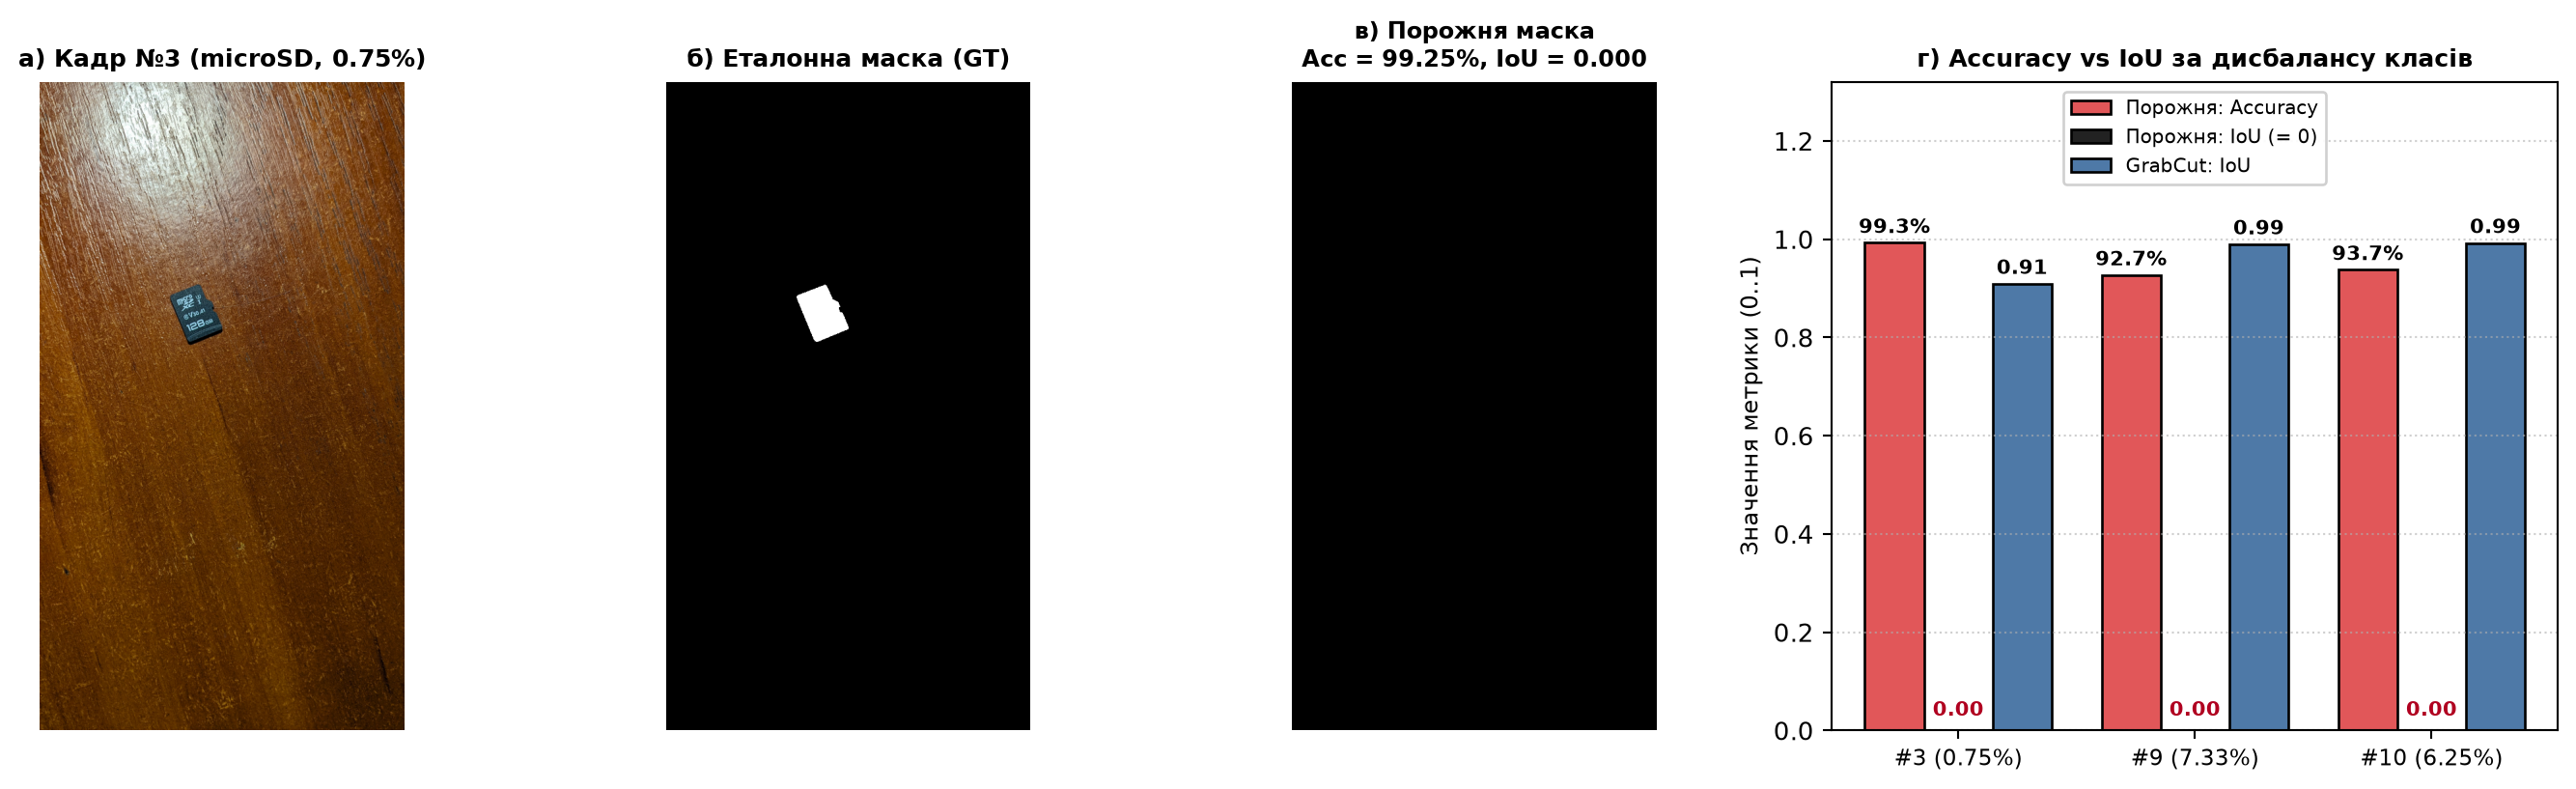
\includegraphics[width=0.98\textwidth]{../figures/c_accuracy_paradox.png}
    \caption{Парадокс піксельної точності за дисбалансу класів (Крок 8): (а--в) кадр №~3 (microSD, $0.75\%$), еталон і порожня маска ($\text{Acc} = 99.25\%$, $\text{IoU} = 0.000$); (г) порівняння $\text{Accuracy}$ і $\text{IoU}$ на трьох малих об'єктах}
    \label{fig:accuracy_paradox}
\end{figure}

\begin{table}[htbp]
\centering
\caption{Оцінювання детектора пішоходів \texttt{HOG+SVM} на 30 кадрах \emph{INRIA Person} ($86$ GT) (Частина E)}
\label{tab:hog_summary}
\scriptsize
\setlength{\tabcolsep}{3.2pt}
\begin{tabularx}{\textwidth}{Y r r r r r r}
\toprule
Конфігурація конвеєра детекції & Детекцій & $\text{TP}$ & $\text{FP}$ & Макс. Recall & Макс. $F_1$ & $\text{AP}$ \\
\midrule
\directlua{tab_hog_summary()}
\bottomrule
\end{tabularx}
\end{table}

\begin{table}[htbp]
\centering
\caption{Залежність метрик детектора \texttt{HOG+SVM} (після \texttt{NMS}) від порога впевненості SVM (Частина E)}
\label{tab:pr_thresholds}
\scriptsize
\setlength{\tabcolsep}{4.0pt}
\begin{tabularx}{\textwidth}{r r r r r r r}
\toprule
Поріг впевненості & Детекцій & $\text{TP}$ & $\text{FP}$ & Precision & Recall & $F_1$ \\
\midrule
\directlua{tab_pr_thresholds()}
\bottomrule
\end{tabularx}
\end{table}

\begin{figure}[htbp]
    \centering
    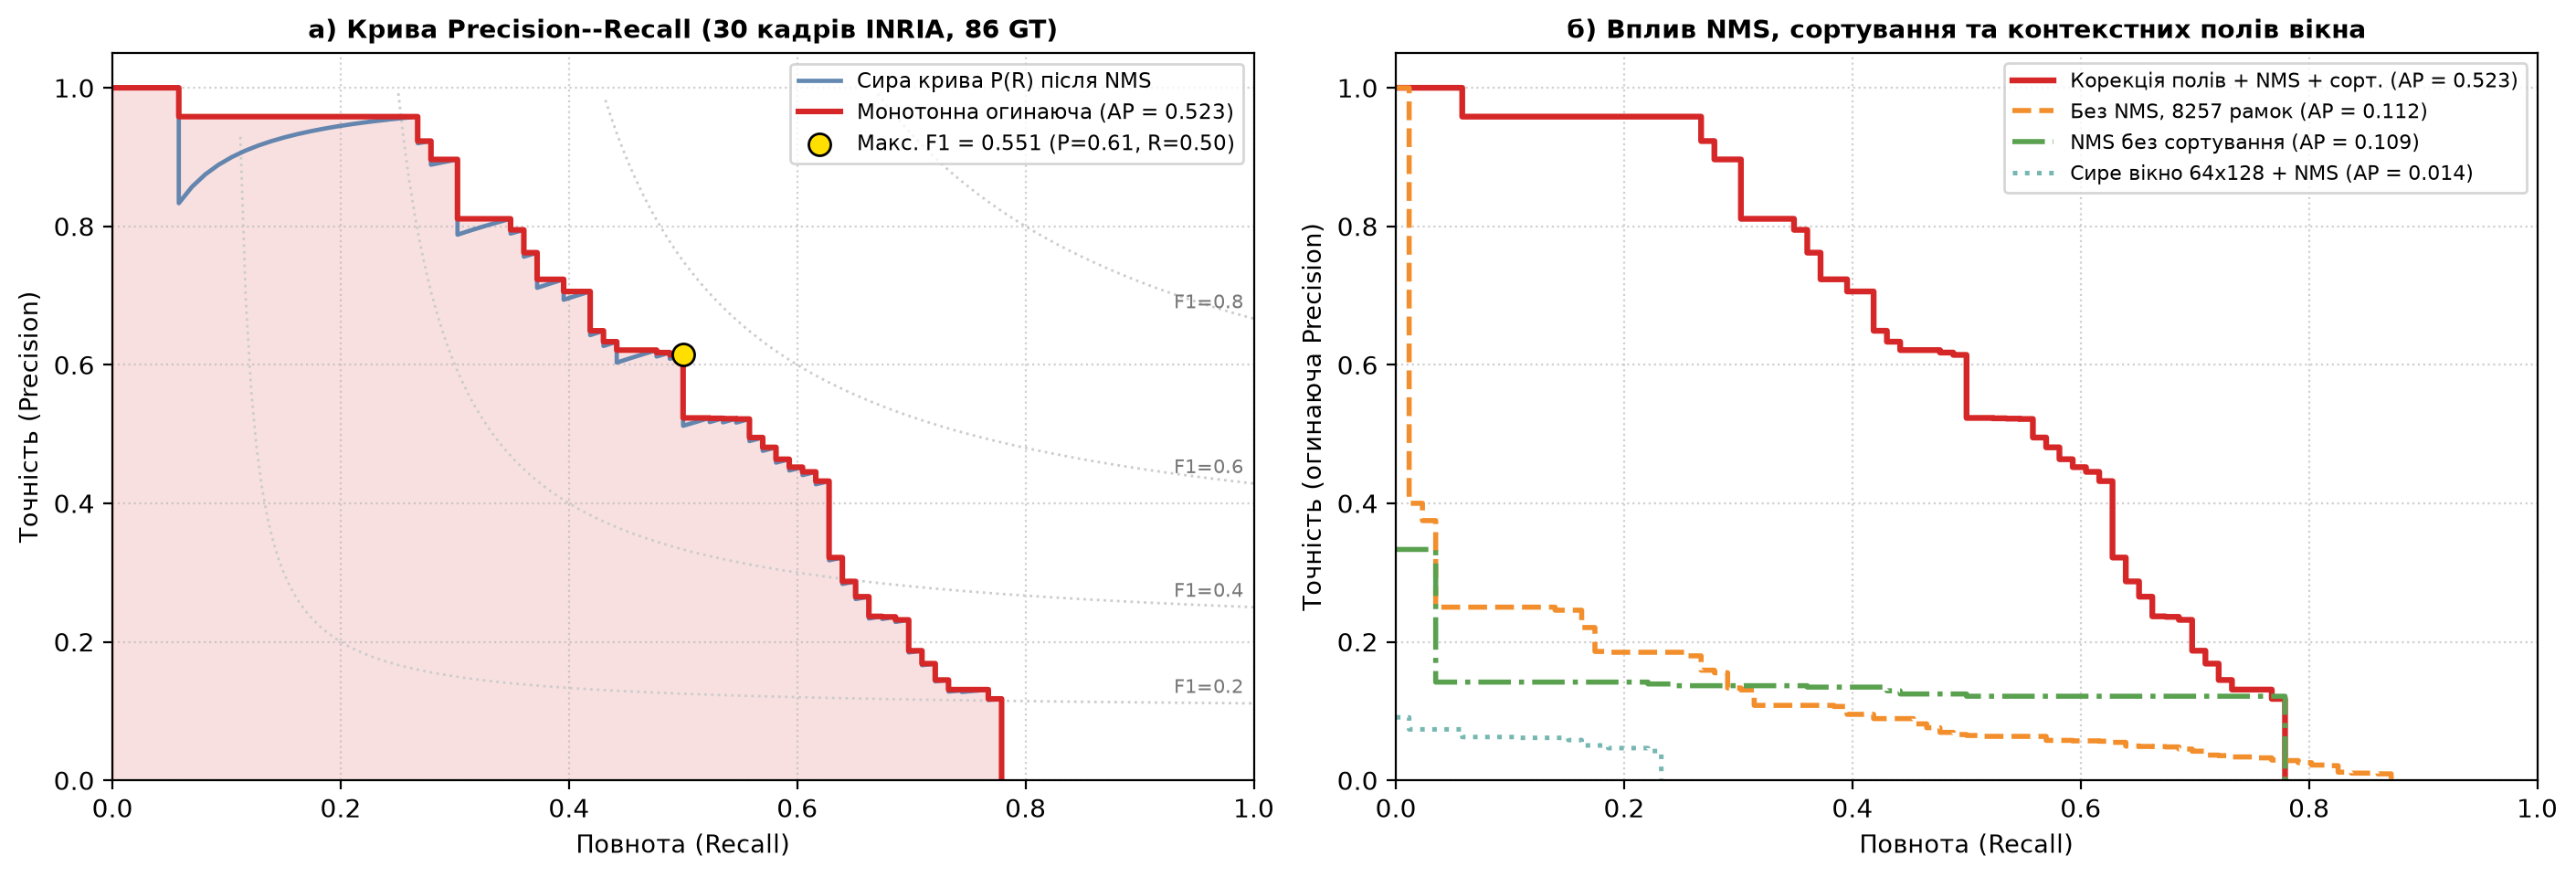
\includegraphics[width=0.98\textwidth]{../figures/e_pr_curve.png}
    \caption{Крива \emph{precision--recall} детектора \texttt{HOG+SVM} на 30 кадрах \emph{INRIA Person} (Кроки 15--16): (а) сира крива, монотонна огинаюча ($\text{AP} = 0.523$) та точка максимуму $F_1$; (б) вплив \texttt{NMS}, сортування та корекції полів вікна}
    \label{fig:pr_curve}
\end{figure}

\begin{figure}[htbp]
    \centering
    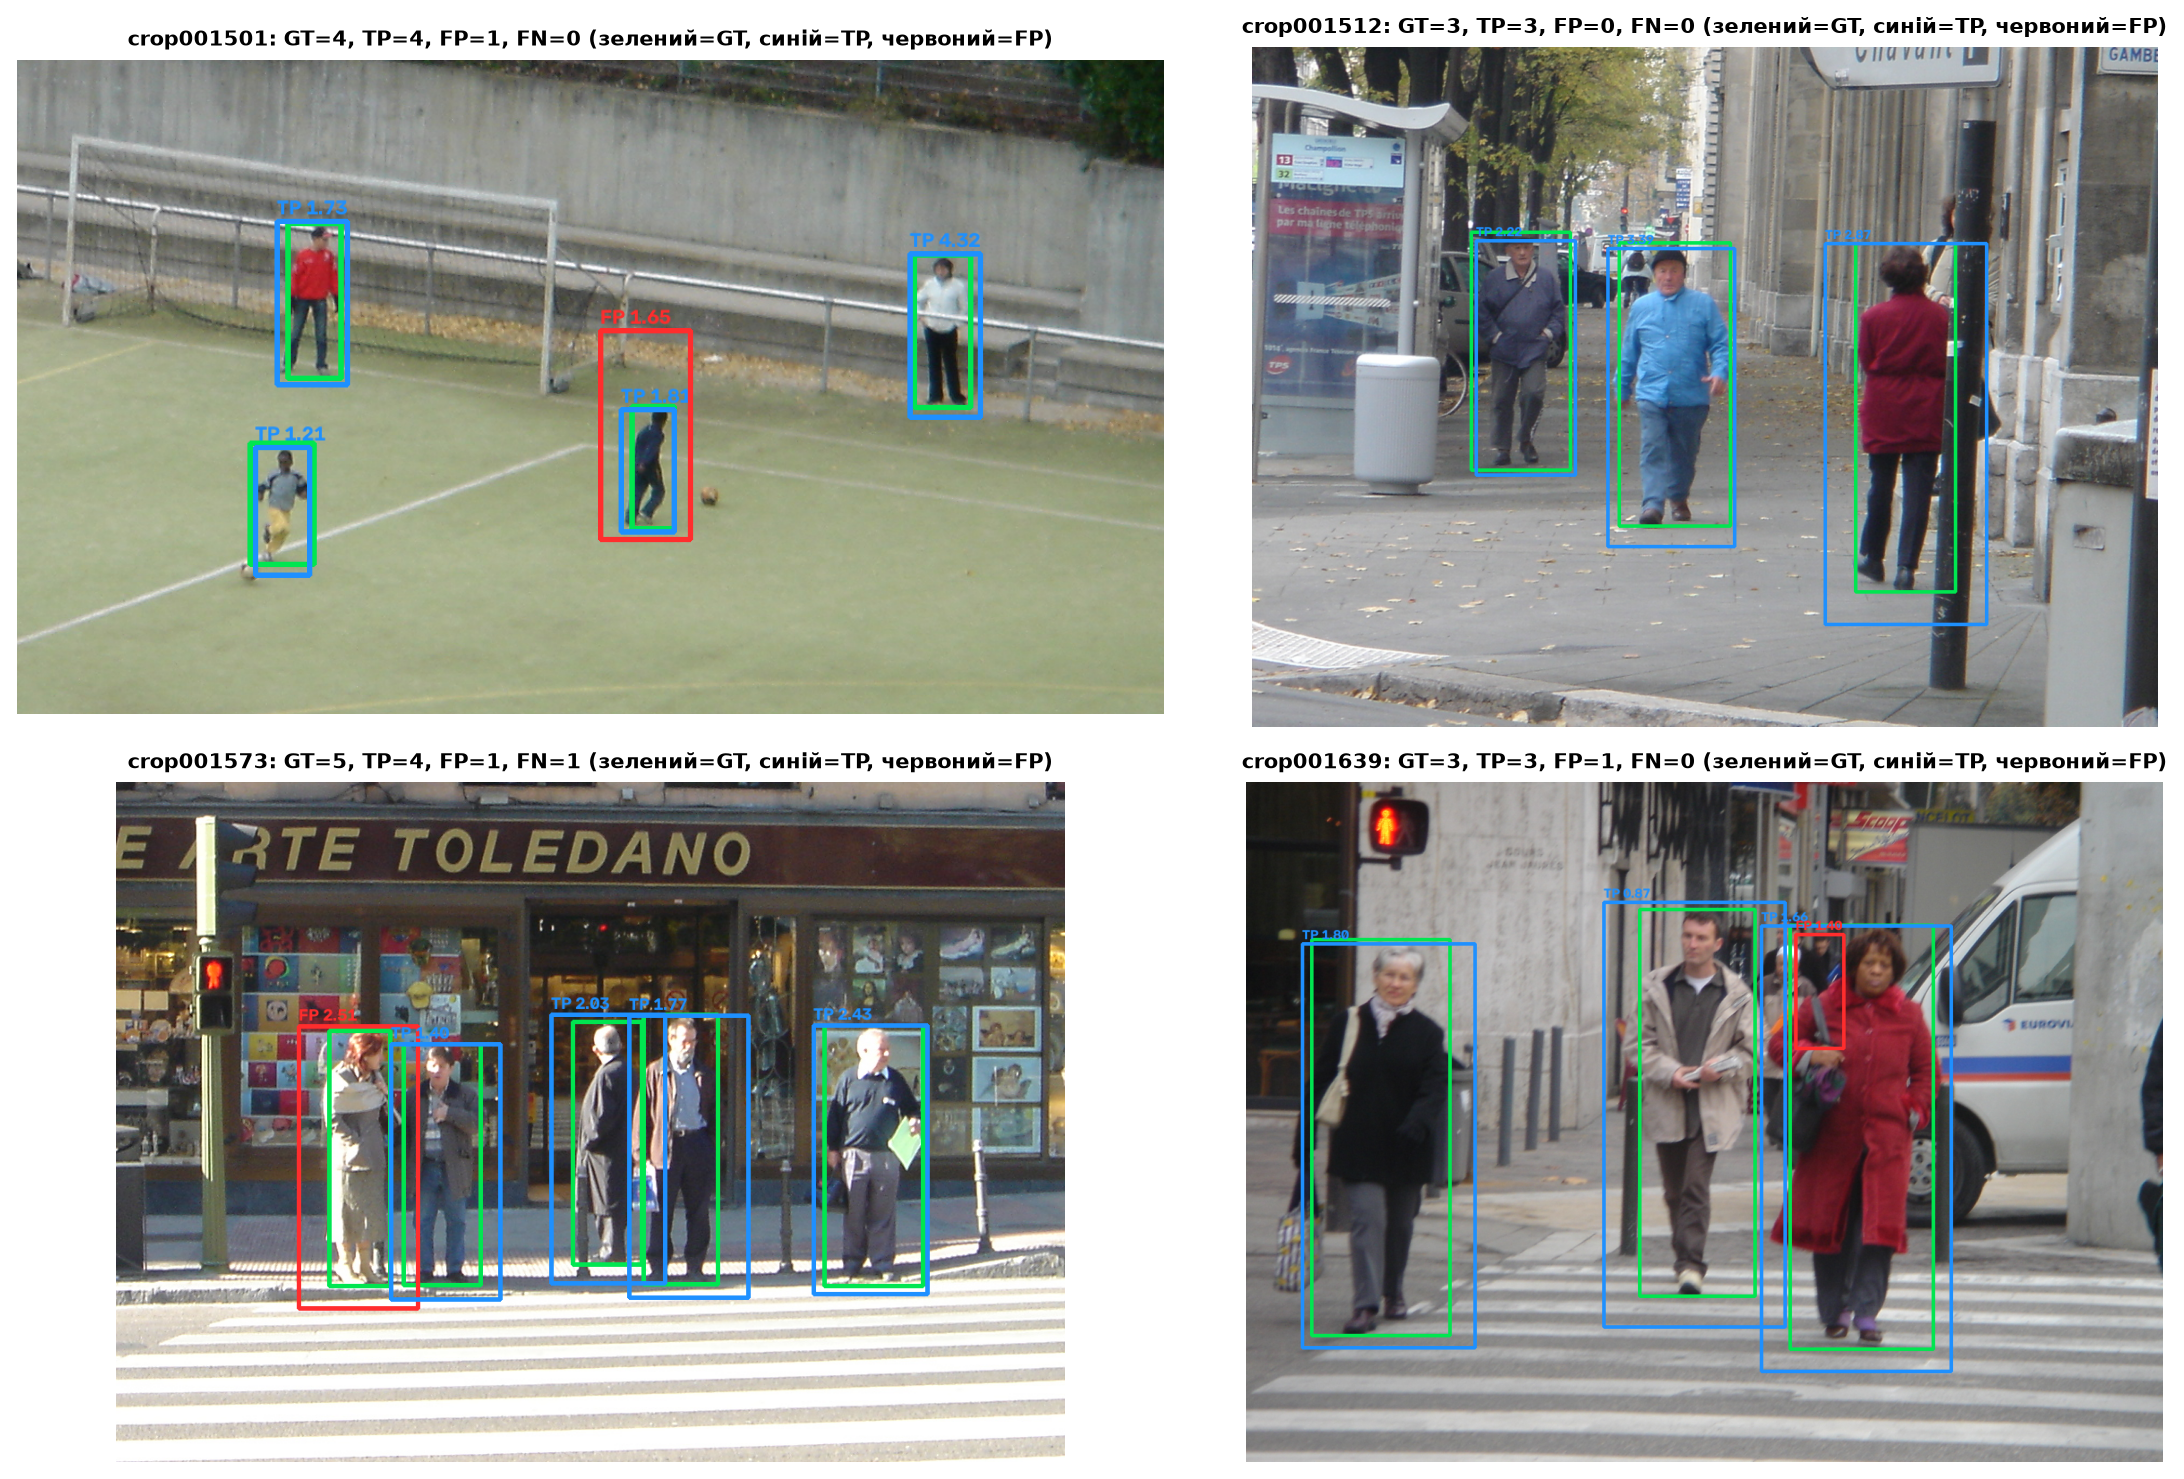
\includegraphics[width=0.98\textwidth]{../figures/e_hog_detections.png}
    \caption{Приклади роботи детектора \texttt{HOG+SVM} після корекції полів і власного \texttt{NMS} при робочому порозі $s \ge 0.87$ (зелений -- еталон GT, синій -- $\text{TP}$, червоний -- $\text{FP}$)}
    \label{fig:hog_detections}
\end{figure}

\clearpage
\section{Аналіз результатів}
\begin{enumerate}
    \item \textbf{Чому середнє $\text{IoU}$ без розкиду вводить в оману (Частина B)}: зведення по всіх 10 зображеннях (Таблиця~\ref{tab:methods_summary}, Рис.~\ref{fig:metrics_boxplot}) безпосередньо ілюструє застереження практикуму. Глобальне порогування Оцу має середнє $\text{IoU} = 0.600$, але величезне стандартне відхилення $\sigma = 0.399$ (діапазон $[0.008; 0.990]$), а маркерний вододіл -- $0.562 \pm 0.432$ ($[0.000; 0.991]$). Пооб'єктна Таблиця~\ref{tab:per_image_iou} пояснює таку бімодальність:
    \begin{itemize}
        \item на п'яти контрастних сценах з однотонним фоном (№~6--10) Оцу та вододіл демонструють високу точність ($\text{IoU} = \mathbf{0.902}$--$\mathbf{0.991}$) за мінімальний час ($2.1$--$13.8$~мс/кадр), зокрема на казу (№~7) вододіл досягає $\mathbf{0.984}$ і перевершує \texttt{GrabCut} ($0.789$), оскільки останній включає в об'єкт м'яку падаючу тінь;
        \item на п'яти складних сценах (№~1--5) глобальні методи повністю відмовляють: у кадрі №~2 (пряжка на лакованому столі) відблиск лампи створює яскравісний градієнт сильніший за контраст об'єкта ($\text{IoU}_{\text{Otsu}} = 0.041$, вододіл -- $0.001$); у кадрі №~3 (microSD, $0.75\%$ площі) гістограма одномодальна і не формує другої моди ($\text{IoU}_{\text{Otsu}} = 0.008$); у кадрах №~1, 4, 5 багатоколірні деталі об'єктів перетинаються за яскравістю з фоном ($\text{IoU} = 0.109$--$0.508$).
    \end{itemize}

    \item \textbf{Порівняння \texttt{SLIC} та \texttt{GrabCut} (Частина B)}: суперпіксельний метод \texttt{SLIC} ($400$ сегментів, $c=10$) із кластеризацією у просторі CIE~Lab знижує розкид ($\sigma = 0.349$), краще тримає межі складних об'єктів порівняно з вододілом (наприклад, на іграшці Ніко №~5: $0.434$ проти $0.109$), але для малих об'єктів (№~9, 10) розмір одного суперпікселя стає порівнянним із границею об'єкта, через що $\text{IoU}$ просідає до $0.710$--$0.787$. Метод \texttt{GrabCut} ($5$ ітерацій) завдяки локалізації рамкою та побудові багатомірних GMM-моделей кольору забезпечує найвищу і найстабільнішу якість на всьому наборі: $\text{IoU} = \mathbf{0.922 \pm 0.079}$ (мінімум $0.789$, максимум $0.993$, $\text{Dice} = 0.958$), проте вимагає $1382$~мс/кадр (у $658\times$ повільніше за Оцу) та чутливий до виражених тіней усередині прямокутника (кадри №~7 і №~8, де $\text{IoU} = 0.789$--$0.792$; Рис.~\ref{fig:seg_comparison}).

    \item \textbf{Оманливість піксельної точності за дисбалансу класів (Частина C)}: на кадрі №~3 (microSD займає лише $0.75\%$ площі, Таблиця~\ref{tab:accuracy_paradox}, Рис.~\ref{fig:accuracy_paradox}) тривіальна порожня маска класифікує $99.25\%$ пікселів «правильно» ($\text{Accuracy} = \mathbf{99.25\%}$), не виявивши жодного пікселя об'єкта ($\text{IoU} = \mathbf{0.000}$, $\text{Dice} = 0.000$). Аналогічний ефект спостерігається на розетці №~9 ($7.33\%$: $\text{Acc} = 92.67\%$, $\text{IoU} = 0.000$) та картці №~10 ($6.25\%$: $\text{Acc} = 93.75\%$, $\text{IoU} = 0.000$). Водночас \texttt{GrabCut} піднімає $\text{Accuracy}$ на кадрі №~3 лише на $0.68$~в.п. (до $99.93\%$), але реально змінює $\text{IoU}$ з $0.000$ до $\mathbf{0.909}$, що доводить необхідність використання саме $\text{IoU}$ або Дайса для задач сегментації.

    \item \textbf{Аналіз конвеєра детекції \texttt{HOG+SVM}, ролі \texttt{NMS}, сортування та контекстних полів (Частина E)}: на 30 тестових кадрах \emph{INRIA Person} ($86$ пішоходів, середній час детекції $528.2 \pm 220.6$~мс/кадр) виявлено три критичні фактори формування коректної кривої \emph{precision--recall} (Таблиці~\ref{tab:hog_summary}--\ref{tab:pr_thresholds}, Рис.~\ref{fig:pr_curve}--\ref{fig:hog_detections}):
    \begin{itemize}
        \item \textit{компенсація контекстних полів вікна Dalal--Triggs $64 \times 128$}: стандартний детектор OpenCV повертає вікно із зовнішніми полями $\sim 16$~пк по периметру, площа якого приблизно вдвічі перевищує щільну еталонну рамку \emph{INRIA}, через що навіть точно центровані детекції отримують $\text{IoU} \approx 0.42$--$0.48 < 0.50$ і формально класифікуються як $\text{FP}$ ($\text{AP} = 0.0142$, $\text{TP} = 20/86$). Відсікання контекстного поля ($16\%$ ширини, $10\%$ висоти) відновлює узгодженість геометрії й підвищує якість у $36.8\times$ -- до $\mathbf{\text{AP} = 0.5230}$ ($\text{TP} = 67/86$, $\text{Recall} = 77.9\%$, макс. $F_1 = 0.551$ при $P = 0.614, R = 0.500, s \ge 0.87$);
        \item \textit{вплив немаксимального придушення (\texttt{NMS})}: без власного \texttt{NMS} (при вимкненому внутрішньому групуванні \texttt{groupThreshold=0}) ковзне вікно генерує $8257$ перекритих рамок, з яких $8182$ стають $\text{FP}$ (бо кожен еталон зіставляється лише раз), обвалюючи $\text{AP}$ у $4.7\times$ -- з $0.5230$ до $\mathbf{0.1121}$. Після \texttt{NMS} ($\text{IoU} > 0.5$) залишається $579$ рамок;
        \item \textit{обов'язковість сортування за впевненістю}: випадковий порядок тих самих $579$ рамок після \texttt{NMS} знижує $\text{AP}$ у $4.8\times$ -- до $\mathbf{0.1091}$, що кількісно підтверджує застереження Кроку~15 практикуму. Основними джерелами помилок при робочому порозі $s \ge 0.87$ (Рис.~\ref{fig:hog_detections}) лишаються дублювання рамок різного масштабу з $\text{IoU} \le 0.5$ та часткові перекриття пішоходів у щільних групах (\texttt{crop001573}).
    \end{itemize}
\end{enumerate}

\section{Висновки}
\begin{enumerate}
    \item Підготовлено та перевірено власний збалансований набір із 10 зображень і строго бінарних масок ($\{0, 255\}$) з об'єктами площею від $0.75\%$ до $34.20\%$ кадру.
    \item Кількісне порівняння 4 методів сегментації показало, що на 10 зображеннях найкращу якість і стабільність забезпечує \texttt{GrabCut} ($\text{IoU} = \mathbf{0.922 \pm 0.079}$, діапазон $[0.789; 0.993]$, $\text{Dice} = 0.958$), тоді як глобальні методи Оцу ($0.600 \pm 0.399$), вододіл ($0.562 \pm 0.432$) та \texttt{SLIC} ($0.560 \pm 0.349$) працюють добре лише на контрастному однотонному фоні ($\text{IoU} = 0.873$--$0.991$), але відмовляють за нерівномірного освітлення й малих об'єктів ($\text{IoU} = 0.000$--$0.041$).
    \item На трьох кадрах із площею об'єкта $<10\%$ експериментально підтверджено парадокс піксельної точності: на карті microSD ($0.75\%$) порожня маска дає $\text{Accuracy} = \mathbf{99.25\%}$ при $\text{IoU} = \mathbf{0.000}$, тоді як \texttt{GrabCut} досягає $\text{IoU} = 0.909$.
    \item Власну реалізацію \texttt{NMS}, зіставлення з еталоном та $\text{AP}$ підтверджено на тесті лекції~8 ($\text{AP} = \mathbf{0.6500}$). На 30 тестових кадрах \emph{INRIA Person} ($86$ пішоходів) детектор \texttt{HOG+SVM} із компенсацією контекстних полів та \texttt{NMS} досяг $\mathbf{\text{AP} = 0.5230}$ (макс. $F_1 = 0.551$); вимкнення \texttt{NMS} знизило $\text{AP}$ до $0.1121$, а відсутність сортування за впевненістю -- до $0.1091$.
    \item Частину~D (узгодженість між розмітниками, Кроки~9--10) програмно підготовлено й буде доповнено фактичним значенням міжрозмітникового $\text{IoU}$ після отримання незалежної маски колеги.
\end{enumerate}

\section{Декларація про використання генеративного ШІ}
Під час виконання даної лабораторної роботи генеративний штучний інтелект (ШІ-асистент Gemini Neon, агентська система Antigravity) використовувався як інструмент парного програмування для автоматизації написання скриптів обчислювальних експериментів із сегментації зображень, власної реалізації \texttt{NMS} та кривої \emph{precision--recall} / $\text{AP}$, побудови візуалізацій і верстки звіту в середовищі LuaLaTeX відповідно до ДСТУ 3008:2015. Усі зображення, ручні маски, числові результати, контрольні перевірки та аналіз випадків відмови зроблено та/або перевірено автором.

\end{document}
